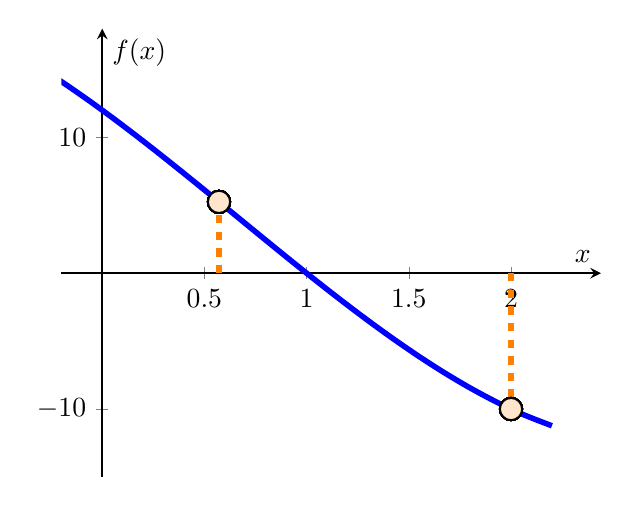
\begin{tikzpicture}
\begin{axis}[axis lines=middle, line width=0.7, enlargelimits=upper, domain=-1:2.2, ymax=15, ymin=-15, xlabel=$x$, ylabel=$f(x)$]
\addplot [smooth, color=blue, line width = 2] {x^3-2*x^2-11*x+12};
\addplot[smooth, color=orange, dashed, line width = 2] coordinates {(2,0) (2,-10)};
\addplot[only marks, mark size=4, color=orange!20, draw=black] (2,-10);
\addplot[smooth, color=orange, dashed, line width = 2] coordinates {(0.5714285714285714,0) (0.5714285714285714,5.247813411078718)};
\addplot[only marks, mark size=4, color=orange!20, draw=black] (0.5714285714285714,5.247813411078718);
\end{axis}
\end{tikzpicture}